\documentclass[a4paper,english,12pt,bibliography=totoc]{scrreprt}

\usepackage[T1]{fontenc} %immer
\usepackage[utf8]{inputenc} %am
\usepackage{babel} %Anfang
\usepackage{comment}
\usepackage{enumitem} %Aufzählungen verändern
\usepackage{natbib} % For bibliography style and citation commands
\usepackage{mhchem} % for chemical formulas
%Gleichungen verwenden
\usepackage{newtxtext}
\usepackage{amsmath}
\usepackage{amssymb}
\usepackage{mathptmx}
%\usepackage{txfonts}

\usepackage{listings}% code blocks
\usepackage[most]{tcolorbox}

%Querverweise
\usepackage{varioref} %immer
\usepackage{hyperref} %in dieser
\usepackage{cleveref} %Reihenfolge

\usepackage{booktabs} %schönere Tabellen
\usepackage{siunitx} %SI-Einheiten
\usepackage{tabularx} %Tabellen mit flexiblen Spalten	

\usepackage{graphicx} %Grafiken verwenden

\usepackage{lipsum} %Blindtext
\usepackage{subcaption}
\usepackage{afterpage}
\usepackage[headsepline]{scrlayer-scrpage} %Paket für Kopfzeilen
\usepackage{afterpage}
\usepackage{float}
\automark[subsection]{section}

\pagestyle{scrheadings}
\ihead{} % oben links
\chead{\leftmark} % oben Mitte
\ohead{} % oben rechts
\cfoot{\pagemark} % unten Mitte
\automark[section]{section} % Modified line

% Zu volle hboxen korrigieren
\tolerance 1414
\hbadness 1414
\emergencystretch 1.5em
\hfuzz 0.3pt
\widowpenalty=10000
\vfuzz \hfuzz
\raggedbottom

%Informationen über das Dokument
\date{\today}


\begin{document}


\begin{titlepage}
	\centering
	
\includegraphics[width=0.8\textwidth]{logo_uulm_sw}
	
	\vspace{1cm}
	\LARGE Laboratory Module for Master Programs
	\Huge \textbf{Biophysics Lab Course}
	
	\vspace{1cm}
	\Large Experiment:

	\Huge \textbf{Optical Tweezers}
	
	\vspace{15mm}
	\Large Performed on 8th May 2024
	
	\vspace{5mm}
	\LARGE Group 8
	
	\vspace{1cm}
	\Large
	\begin{tabular}{rcl}
	\textbf{Haiyang Zhang} & and & \textbf{Nicolae Turcan}\\
	\href{mailto:student.1@uni-ulm.de}{haiyang.zhang@uni-ulm.de} & & \href{mailto:student.2@uni-ulm.de}{nicolae.turcan@uni-ulm.de}
	\end{tabular}
	
	\vspace{7mm}
	Supervisor: Tobias Bischof 
	
	\vfill
	\begin{tabular}{p{50mm}@{\hspace{5cm}}p{50mm}}
	\hrulefill & \hrulefill \\
	%\centering Haiyang Zhang  & \centering Nicolae Turcan
	\end{tabular}
	
	\vspace{5mm}
	\normalsize \raggedright
	We hereby confirm that we have elaborated the present work independently and have detailed knowledge of the entire contents.
\end{titlepage}



\tableofcontents

\chapter{Introduction}
\label{cha:Introduction}

The bacterial flagellar motor (section 1.1) controls the motion of the flagellum by producing a force of a few piconewtons, causing a conformational change in the flagellum of several nanometers. Optical tweezers (section 1.2) is a tool consisting of a focused laser beam able to manipulate microscopic particles precisely. In this experiment, we employed optical tweezers to explore the torque generated by the flagellar motor of E.coli.


\section{Bacterial flagellar motor}

\begin{figure}[H]
    \centering
    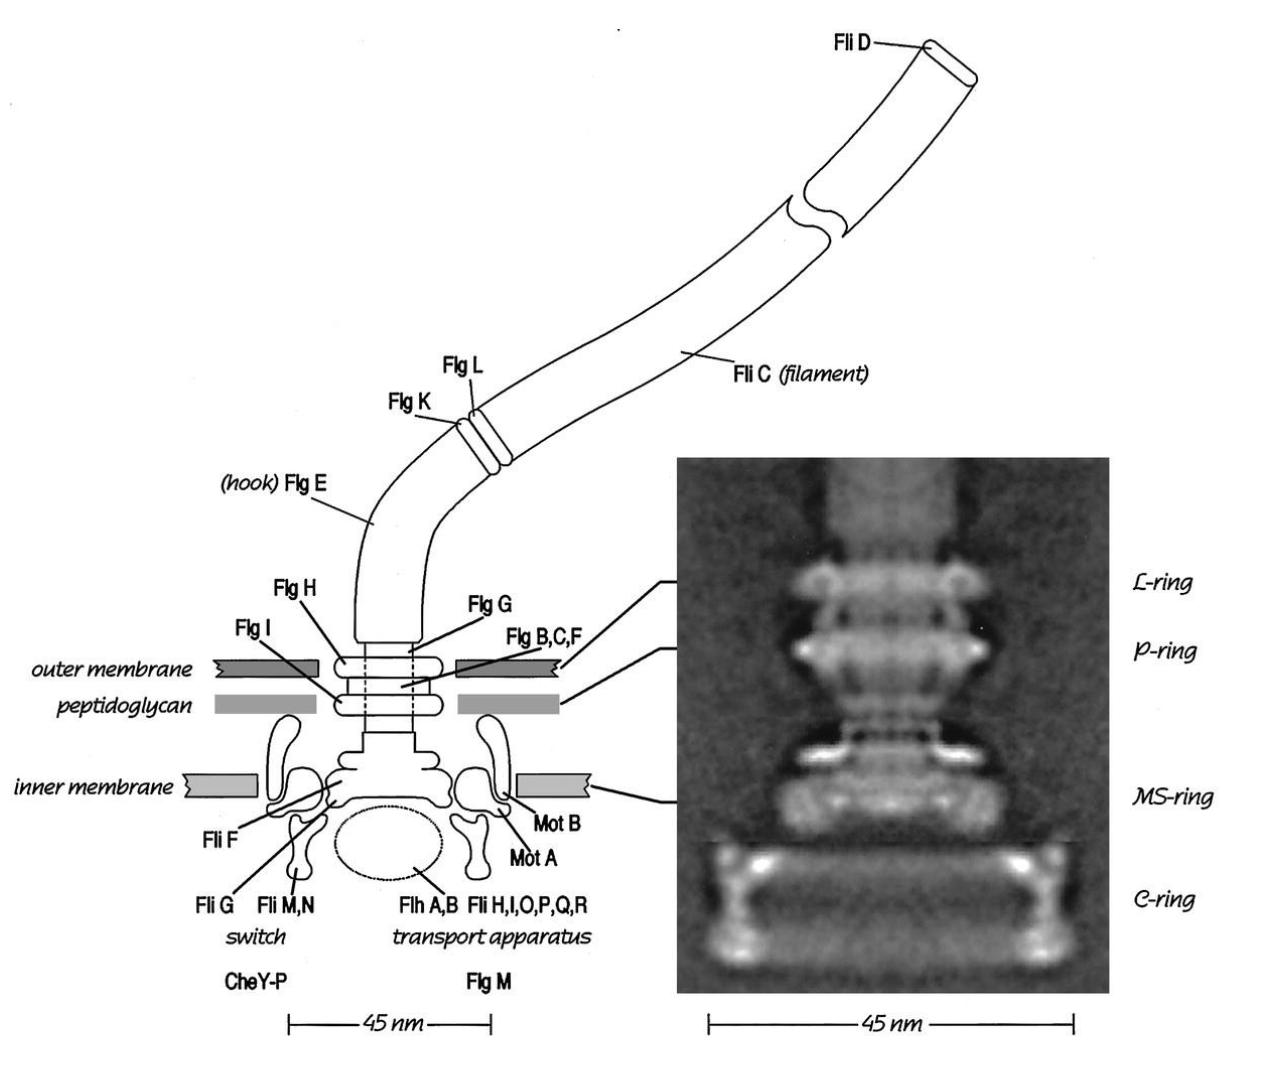
\includegraphics[width = 0.75\textwidth]{Images/flagellar motor.png}
    \caption{structure of the flagellar motor\cite{lab_manual}}
\end{figure}

Flagellae are thread-like extensions used for bacterial locomtion. They are located on the cell's surface and connected to the rotational molecular motor called bacterial flagellar motors. As is shown in Figure 1.1, the motor consists of two parts, the stator and the rotor. The stator (Mot A \& B part) is anchored to the plasma membrane and it is composed of 8 subunits with at least one proton channel in each. The structure of the stator makes it possible for bacterial flagellar motors to use the  \ce{H+} ion gradient as the energy source \cite{fung_powering_1995}. The rotor(FliG, FliM, and FliN) is connected to the helical flagellum and can rotate the flagellum.\\

The bacterial flagellar motor determines the movement of the bacterium by the direction of rotation. For example E.coli moves forward using a counterclockwise rotation which creates a bundle of flagellae that move in synchrony. While the flagellum rotates clockwise, the bundle falls apart so the directed movement stops and another type of movement begins ,the bacteria tumbles more or less chaotically. The chemo-receptors on the bacteria's surface will check the concentration of the nutrients or harmful substances in the environment to sustain a positive-feedback loop or a negative one, this process is defined as chemotaxis . In conclusion, understanding the rotation of the motor helps us to understand the movement of bacteria at this microscopic scale.

\section{Optical tweezers}
\begin{figure}[H]
    \centering
    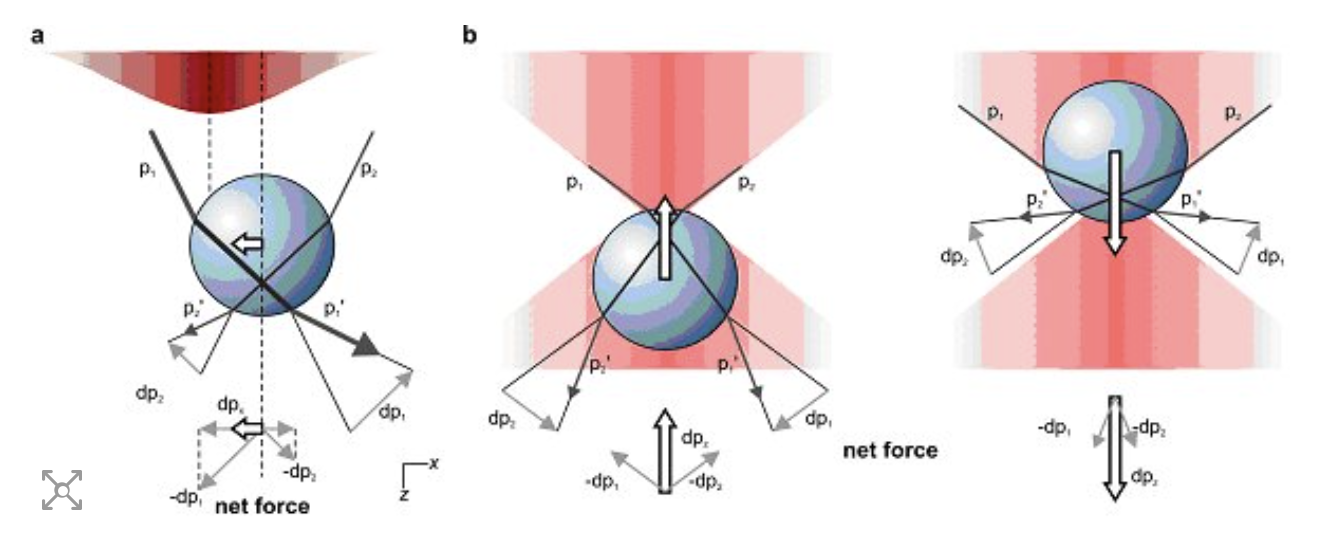
\includegraphics[width = 0.8\textwidth]{Images/Opt.png}
    \caption{The principle of optical tweezers\cite{physics_world}}
\end{figure}
Optical tweezers use light to capture and manipulate microparticles. It can exert a force on the particle through the momentum of light, this momuntum can be used to exert a force only if there is a difference between the refractive index of the environment and that of the particle. As is shown in Figure 1.2.A, a laser with Gaussian intensity can apply a force on the bead. With a focused laser(Figure 1.2.B), the movement of the bead will induce a resisting force and trap the bead in a certain position.\\

If we  use the optical tweezers to displace the bead trough a medium, the force on the bead applied by the optical tweezers will follow Hook's law. However  if the external force on the bead is larger than the force applied by the optical tweezers, the bead will escape. This maximum force is called escape force.

\chapter{Experiment and results}
\label{cha:Experiment}

\section{Optical setup}
The optical set-up of this experiment is described in detail in Figure 2.1.\\
\begin{figure}[H]
    \centering
    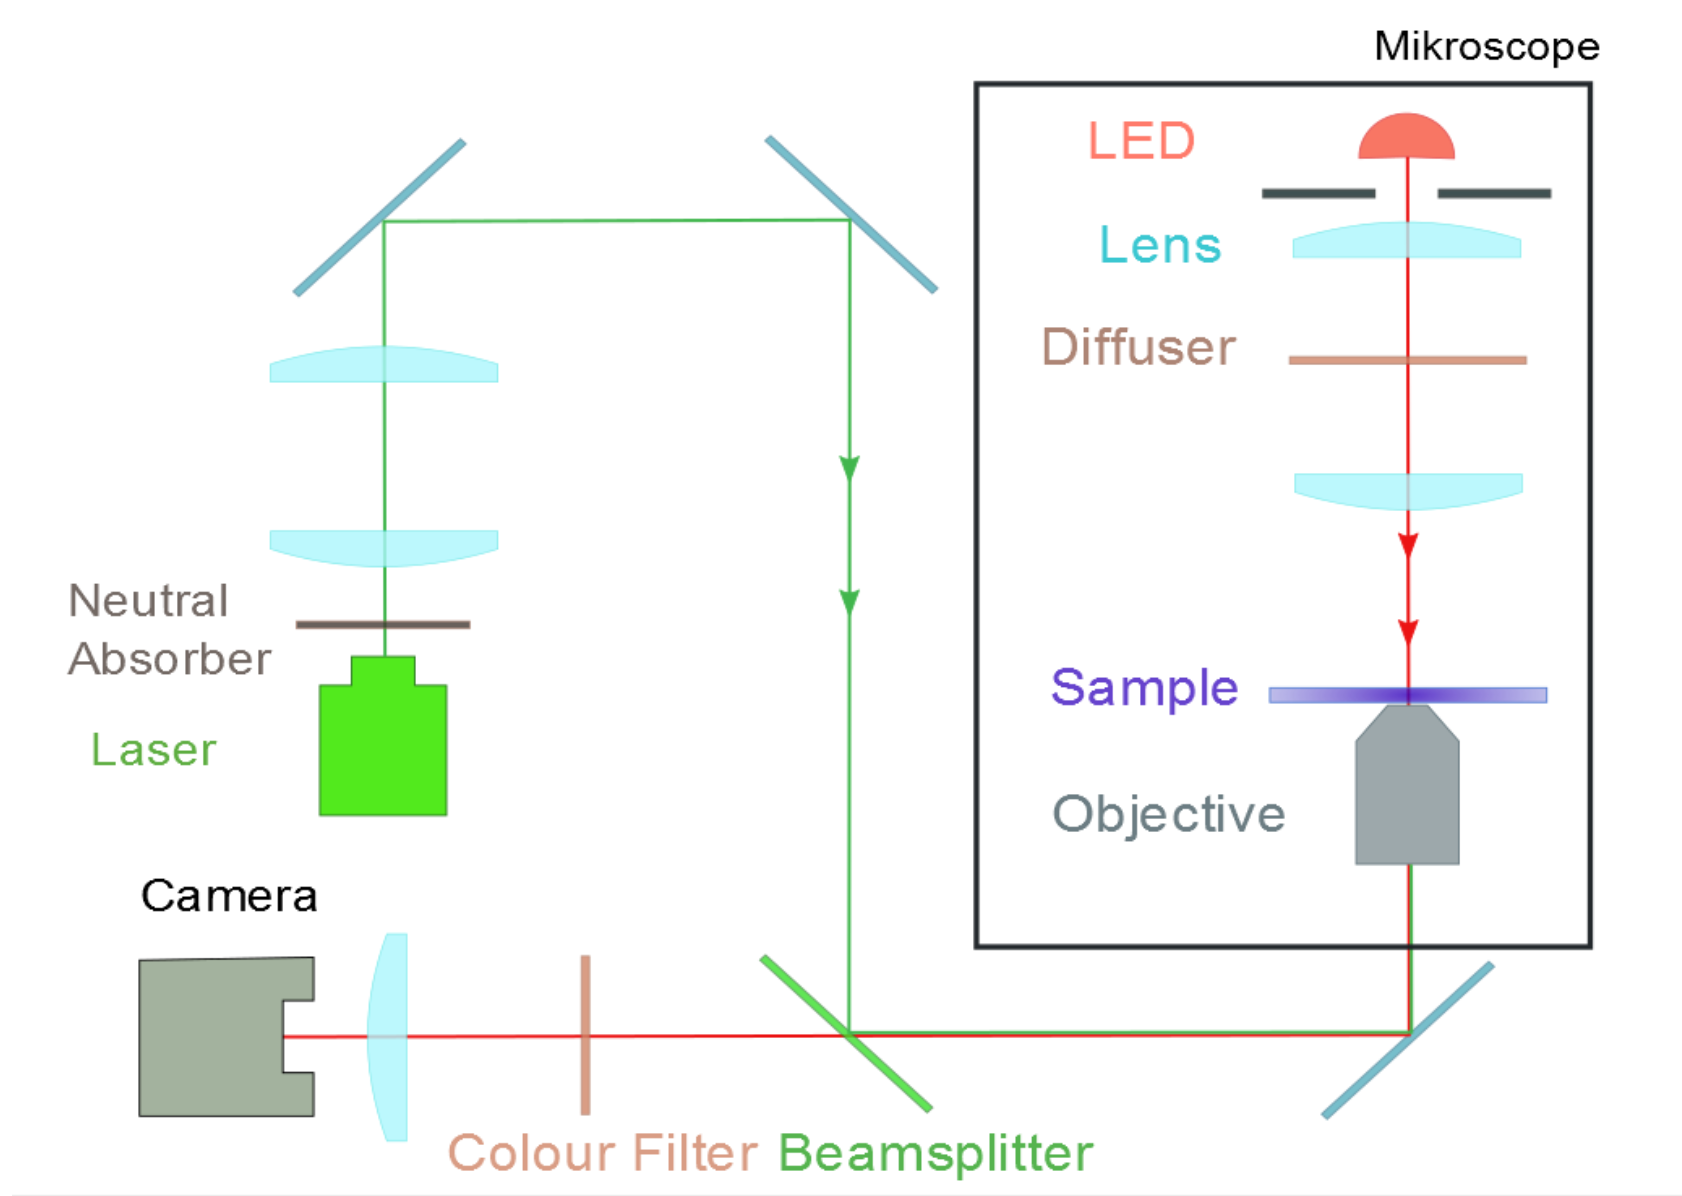
\includegraphics[width = 0.8\textwidth]{Images/experiment setup.png}
    \caption{Optical set-up of the experiment\cite{lab_manual}}
    \label{fig:enter-label}
\end{figure}
A  class III laser of 532 nm is used for the creation of the optical trap, considering the high-intensity laser, a neutral density filter with OD = 0.6 is used to decrease the intensity of the beam. Following is mounted a beam expander and collimator to make use of the full back aperture of the objective when focusing the beam. Two mirrors mounted on kinematic mounts, with control over 3 axes allow for the correct positioning of the beam. In the setup, the beam splitter and color filter were substituted by a dichroic mirror.\\

The objective employed is a 100x Oil-immersion objective with a Numerical Aperture of 1.3 which will be used for both Optical trapping and view.\\

The widefield microscopy setup consists of a red LED and piece of paper that acts as diffuser, followed by a condenser to allow proper illumination of the sample.\\

The camera is a Thorlabs sensor without a Bayer filter running at 20fps.
The Dataset was recorded at 20fps, meaning 1 image was recorded in the .tiff file for every 20ms.
The Stage is controlled in XY directions by a joystick and usb-COM commands.


\section{Microscope Calibration}
The image formed by the Setup was calibrated with a Thorlabs slide containing perpendicular lines every 10 µm \cite{noauthor_thorlabs_nodate} to achieve a conversion value between pixels and µm.
The image was analyzed in FIJI \cite{schindelin_j_arganda-carreras_i_frise_e_kaynig_v_longair_m_pietzsch_t__cardona_a_fiji_2012} which allowed us to do multiple measurements and define a mean value of 118,268 nm/pixel.
Careful consideration was taken into correctly focusing the objective on the lines and mounting and demounting of the slides to avoid damage to the objective.
\begin{table}[h]
\centering
\caption{Measurements}
\begin{tabular}{@{}ll@{}}
\toprule
Measurement & Pixels = 70µm \\ \midrule
1           & 590,464         \\
2           & 590,731         \\
3           & 590,730         \\ \bottomrule
\end{tabular}
\end{table}

\section{Optical tweezers calibration}

To perform a calibration of the optical tweezers that could in turn allow us to convert laser intensity in a pN value , we used 2µm polystyrene beads suspended in a mounting solution between 2 slides glued together with bi-adhesive tape forming a thin channel.
The ends of the channel were closed with nail polish to prevent evaporation.
The conversion of a laser intensity into a force is enabled by the considering that the escape force of optical tweezers can be equal to the force applied by viscous friction in a flow with opposite direction. We want to find the Laser Intensities for which the Formula under here is true.
\[
F_0 = F_f
\]
Now we know that the frictional force of a stationary object in a fluid can be described as:
\[
F_f =\beta v
\]
where $\beta$ is the friction coefficient and v is the velocity. The friction coefficient can be computed as follows: 
\[
\beta = 6\pi\eta r.
\]
where r is 2$\mu$m  and $\eta$ is the viscosity of water at 20°C is  roughly 1 mPa⋅s.

Finally, we must consider that the objective has a very short working distance and that the polystyrene beads are close to the coverglass surface, therefore we need to introduce a correction factor as follows, where we assume h to be 0.03mm:

\[
\beta = \frac{6 \pi \eta r}{1-\frac{9}{16} \frac{r}{h} + \frac{1}{8} {(\frac{r}{h})}^3 - \frac{45}{256} {(\frac{r}{h})}^4 - \frac{1}{16}{(\frac{r}{h})}^5}
\]

\begin{figure}[htbp]
\centering
\begin{minipage}[t]{0.48\textwidth}
\centering
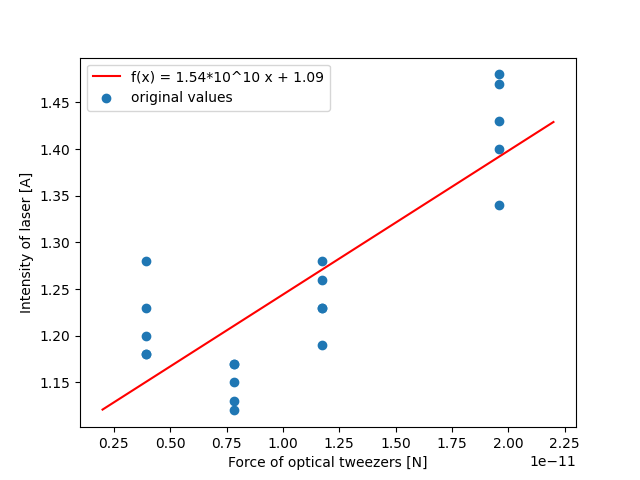
\includegraphics[width=6cm]{Images/fitting1.png}
\caption{The fitting with all the data, \\R^2 = 0.5142}
\end{minipage}
\begin{minipage}[t]{0.48\textwidth}
\centering
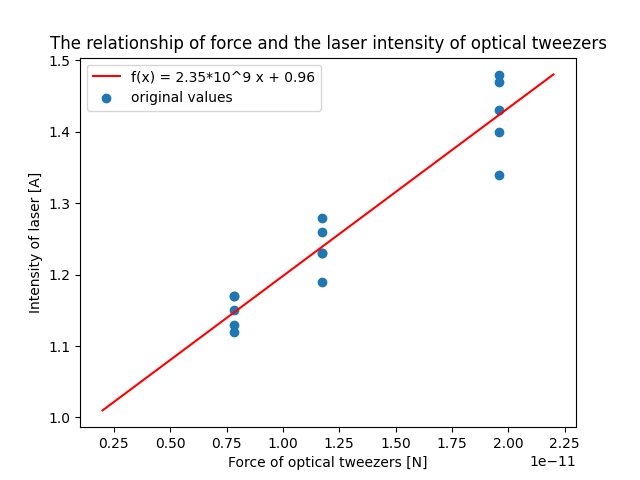
\includegraphics[width=6cm]{Images/fitting2.png}
\caption{The fitting with speed 0.2, 0.3 and 0.5, R^2 = 0.9005}
\end{minipage}
\end{figure}

In conclusion, we can compute the forces corresponding to the measured light intensities by trapping a polystyrene bead and dragging it at a constant velocity( trough the use of a computer command to the stage), and decreasing the light intensity until the bead is lost.
When the bead is lost, an equilibrium between the frictional force and 
the the force of optical tweezers is achieved. Multiple measurement are done for each velocity to achieve statistical significance, and by fitting the data we got the linear relationship between the laser intensity and the optical tweezers force. Thus we can know the force given by the optical tweezers with the laser intensity recorded during the experiment.\\

As the $R^2$ value pointed out in our fitting, the first group of data(v = 0.1mm/s) could be an outlier caused by the experimental operation error(See discussion). In the following calculation, we applied the fitting result shown in Figure 2.3.
%R_1 = 0.5142 , R_2 = 0.9005
\section{Torque of bacterial flagellar motor}

Two different methods(balancing the motor torque with viscosity, and balancing the motor torque with optical tweezers) were applied to measure the torque of the bacterial flagella motor.\\

In the first method, the force of optical tweezers was set to 0, and the only two torques on the bacteria were the force generated by bacterial motor M and the viscosity V. While the two torque are balanced(V = M), the bacteria will rotate under a constant angular velocity. Thus, by calculating the torque given by the viscosity using the following formulas, we can acquire the torque generated by the molecular motor. Here, we approximated the bacteria as an ellipse for our calculation. \\

\[ Viscosity: M = \beta_r \omega
\]
 \[
 \beta_r = \beta_{sphere} \alpha
 \]
 \[
 \beta_{sphere} = 6\eta \frac{4}{3} \pi a b^2
 \]
 \[
 p = b/a
 \]
 \[
 \alpha = \frac{4}{3} \frac{1-p^4}{p^2(-2-p^2S+2S)}
 \]
\[
S = \frac{2}{\sqrt{1-p^2}} ln[\frac{1}{p}(1+\sqrt{1-p^2})]
\]

In the experiment, we recorded 9 movies, in which we acquired the angular velocity $\omega$ of bacteria , the semi-major axis a and the semi-minor axis b(Table 2.2).

\begin{table}[H]
    \centering
    \begin{tabular}{|c|c|c|c|c|}
    \hline
         Number&angular Velocity[rad/s]& semi-major axis [nm]&semi-minor axis [nm]& torque[pN $\cdot$ nm] ]\\
         \hline
         1&5.86 &1282.38 &329.67 &60.72 \\ 
         \hline
         2&2.63 &1746.75 &573.77 &82.01 \\ 
         \hline
         3&4.68 &1412.11 &353.26 &63.56 \\
         \hline
         4&2.54 &1996.89 &222.63 &64.30 \\ 
         \hline
         5&7.51 &2076.07 &704.76 &402.77 \\ 
         \hline
         6&7.45 &1821.91 &471.95 &222.45 \\ 
         \hline
         7&13.33&886.47  &358.11 &64.43 \\ 
         \hline
         8&4.68 &1493.66 &415.59 &80.72 \\ 
         \hline
         9&8.14 &1691.40 &386.50 &179.67 \\ 
         \hline
    \end{tabular}
    \caption{The angular velocity, geometric parameters of bacterium and the torque \\under V = M}
    \label{tab:my_label}
\end{table}

In our second method, we attempted to capture the rotating bacteria with optical tweezers, and then we lowered the intensity of the laser until the bacteria moved again. At the critical point of the bacteria started moving, the torque generated by the optical tweezers(T) was equal to the torque given by the bacterial motor(M).The force of the optical tweezers was recorded. We assume that the bacterium which could move again was not destroyed by the laser beam, so their motor could still generate the same order of force even if they were captured by the optical tweezers. \\

By assuming the lever arm of the optical tweezers is 2/3 of the bacteria length, we could calculate the torque given by the optical tweezers, also the torque of bacterial motor(Table 2.3). In the experiment, unfortunely, most of the bacteria passed away or could not perfectly function after being captured by the optical tweezers. The best result(not listed in table 2.3) could get captured and successfully escape from the optical tweezers several times, under the laser intensity of 1.04 A, the estimated torque from this measurement was 7707.66 pN$\cdot$ nm.

\begin{table}[H]
    \centering
    \begin{tabular}{|c|c|c|c|}
    \hline
intensity [A] & lever arm distance [nm] & force [pN] & torque[pN $\cdot$ nm]\\
            \hline
             1.2&1709.41 &10.08 & 17230.93\\
             \hline
             1.55&2328.42 &24.96 &58111.07\\
             \hline
             1.08&1882.45 &4.98 &9372.80\\
             \hline
             1.08&2661.85 &4.98 &13254.19\\
             \hline
             1.205&2767.40 &10.29 &28483.75\\
             \hline
             1.05&2428.61 &3.70 &8995.86\\
             \hline
             1.08&1181.67 &4.98 &5883.91\\
             \hline
             1.06&1991.05 &4.13 &8221.41\\
             \hline
             1.087&2254.64 &5.28 &11897.42\\
             \hline
    \end{tabular}
    \caption{The geometric parameters and the torque of bacterium under T = M}
    \label{tab:my_label}
\end{table}

\section{ Testing for normality of trap dwell times at Equilibrium}

The following considerations apply only to recording 31, for which a video was taken for for 48.7 Seconds under a constant light intensity produced by 1.04 A, this was considered to reach an equilibrium and the arguments supporting this novel method are expressed in the discussion, as described above the bacterium escaped multiple times and the torque generated was 7707.66 pN$\cdot$ nm. \\

Consider the case in which the force that the flagellum can exert depends on a gradient difference in \ce{H+}Ion concentrations, if the flagellum is stopped, then the Ion concentration  increases linearly until it is able to overcome the force applied by the trap, which in turn should always require the same amount of time because of the linear relationship between gradient concentration and time. \cite{biquet-bisquert_dynamic_2021} \\
In the case in which the two forces actually equal each other ( an Equilibrium), escaping the trap can only be possible thanks to external forces, which at this scale we describe as Brownian Motion, which is inherently random. Meaning that the escape time required should be random instead of normally distributed around a mean value.

The QQ plot below shows that the datapoints recorded do not sit close to the line representing an hypothetical normal distribution,  alongside we present a histogram of the recorded distribution compared to a normal distribution and a computed density  distribution, the tests were implemented in R and are available in the Supplementary Material.
\\

\begin{figure}[htbp]
    \centering
    \begin{subfigure}[b]{0.49\textwidth}
        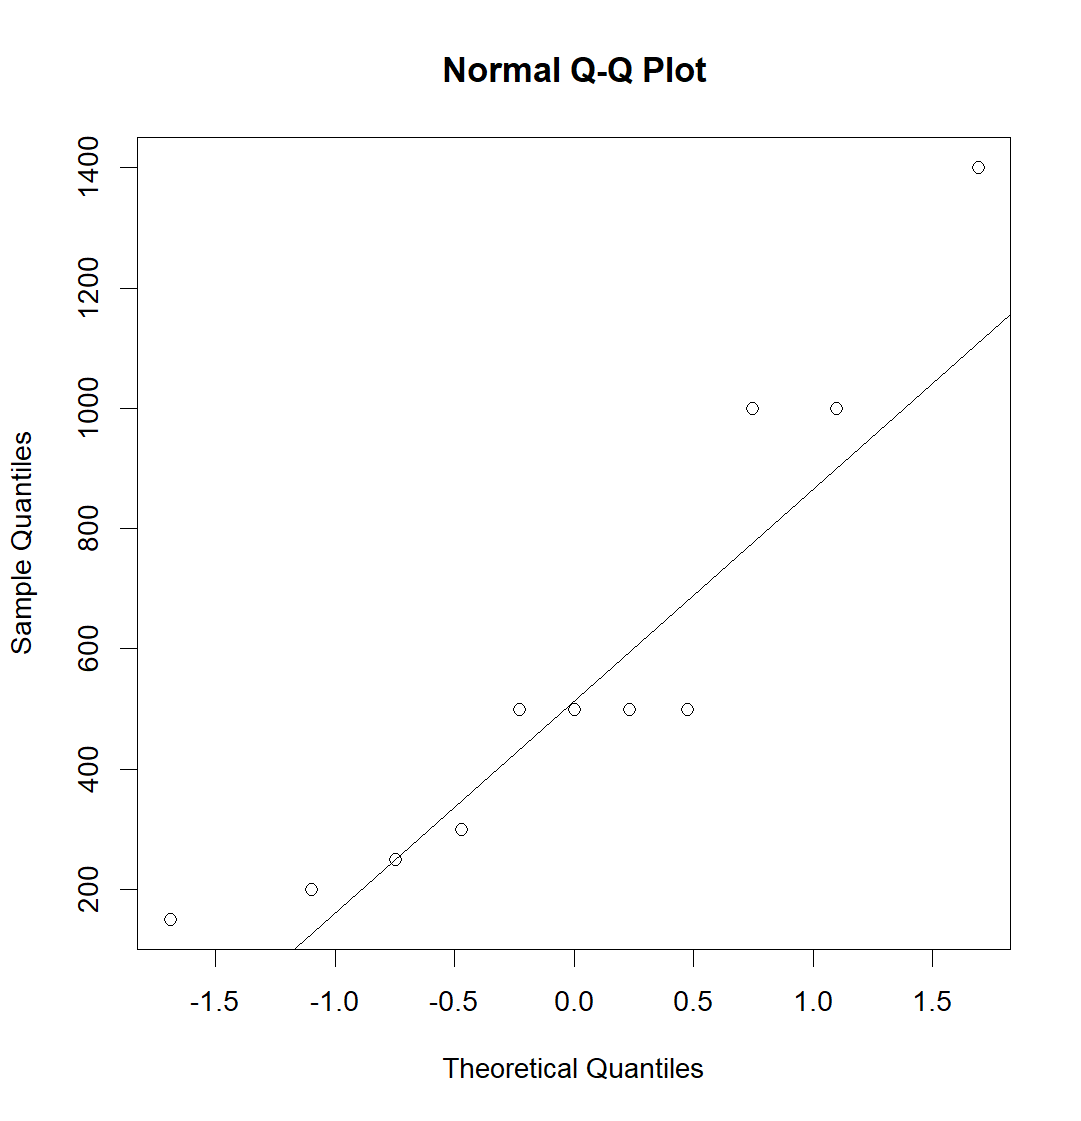
\includegraphics[width=\textwidth]{Images/qqplot.png}
        \caption{QQ plot }
        \label{fig:figure1}
    \end{subfigure}
    \hfill
    \begin{subfigure}[b]{0.49\textwidth}
        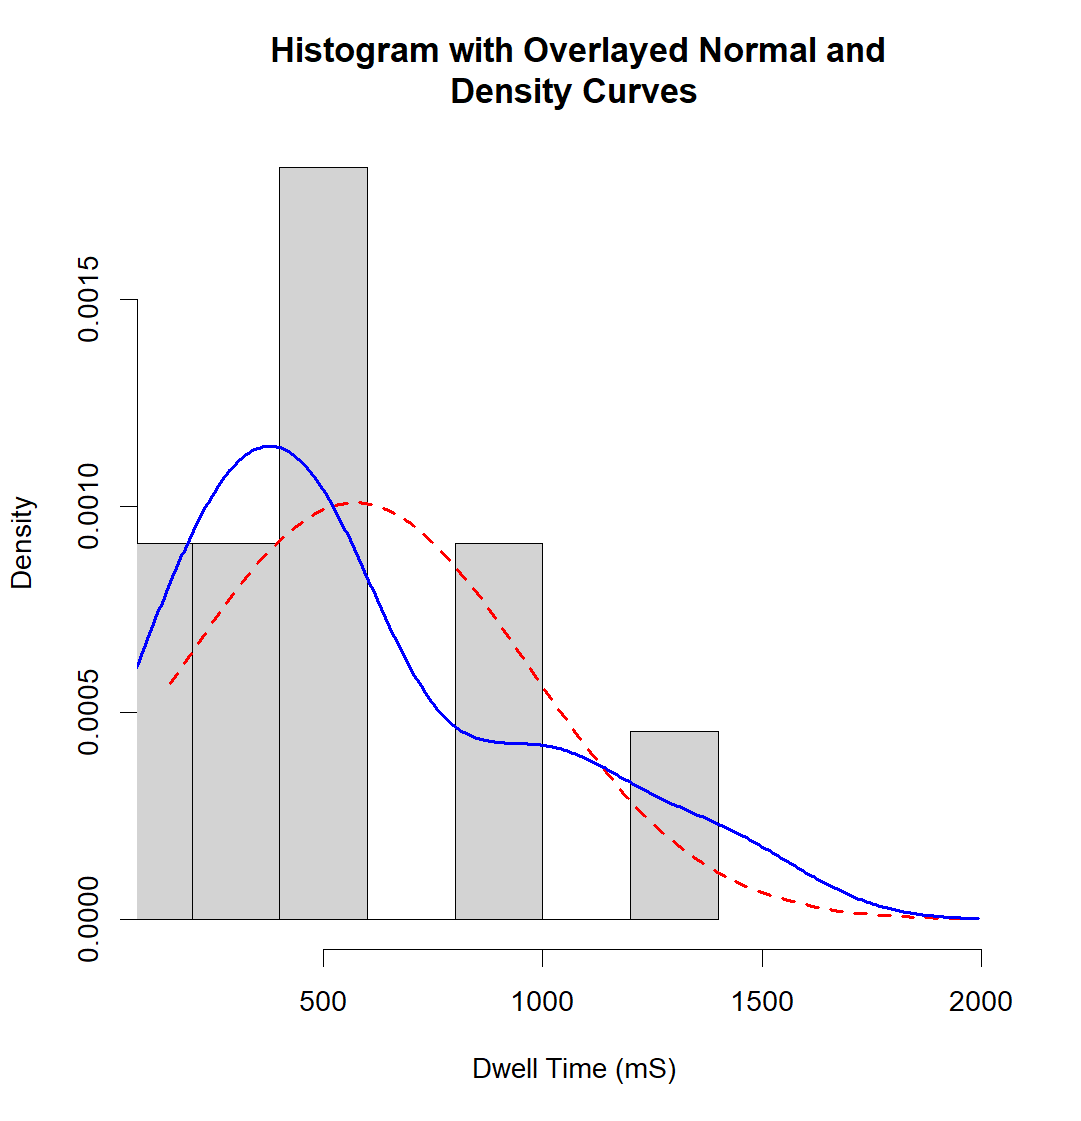
\includegraphics[width=\textwidth]{histogram.png}
        \caption{Histogram}
        \label{fig:figure2}
    \end{subfigure}
    \caption{}
    \label{fig:both_figures}
\end{figure}

We also performed a Shapiro-Wilk test \cite{shapiro_analysis_1965} for Normality  and the results are presented in the following Table 2.3.

\begin{table}[H]
\centering
\caption{Shapiro-Wilk Test for Normality}
\begin{tabular}{|c|c|}
\hline
Test Statistic & Value \\
\hline
W & 0.86385 \\
p-value & 0.06458 \\
\hline
\end{tabular}
\end{table}

The W statistic is only positive and represents the difference between the estimated model ( a normal distribution) and the observations. The presented W values suggests that a normal distribution doesn´t represent well our data.
And considering that the Shapiro-Wilk test uses only the right-tailed test we use an $\alpha$ value of 0.10, for a 95\% confidence interval, and for this reason we can confirm that the p-value of the Shapiro-Wilk Test can be interpreted as a confirmation that our data is Randomly distributed.\\

We can therefore state that the data is inherently random and a true equilibrium of forces between flagellum torque and optical trap was achieved.


\chapter{Discussion}
\label{cha:Discussion}



% We removed the datapoints for the speed of 0.1 m/s since they dindn´t fit in a linear regression, this was required because we work on the assumption that laser intensity is linear.
During the analysis of the escape force from the optical tweezers, the datapoints corresponding to the velocity of 0.1 mm/s were removed because in contrast with the assumption that the laser intensity has a linear relationship with the force generated. The argument proposed for this discrepancy is that our ignorance of the instrument altered the first measurements.\\


%- a note on scattering and that beads are lost if they are behind the focus and pushed in place if in front or close-by 

During the experiment, we noted that some particles wouldn´t get trapped inside the Optical Well, it was pointed to us that only particles in front of the focal point could get trapped and those behind the focal point of the optical tweezers wouldn´t feel any force pushing them towards the focus.
This can be attributed to the fact that the possible optical pathways described in Figure 1.2 do not describe scattering.
Scattering is a process through which the photon is elastically scattered and emitted in a random direction, with some distribution around an axis, and if we assume the case in which the majority of photons are scattered forward another force is being applied to the particle, and it is thus possible that our particle is pushed away with a vector greater than the one described in Fig. 1.2(c).
This effect resulted in the need to prepare multiple slides containing polystyrene beads for the calibration process.\\

%- a note on how light significantly slowed/ killed bacteria 
During the measurement of the forces generated by the flagellar motors we encountered many times a recurrence that couldn´t be described quantitatively in our analysis, but the effect of which was quite evident and could result in a significant bias of the results. The bacteria subjected to a high intensity illumination by the optical tweezers were significantly slower in their turning rate, even after the illumination was removed. In fact many of the candidate bacteria stopped completely after this process, in what we considered to be death.
This was the case for the majority of the bacteria we recorded, roughly 2/3 of the total recordings were excluded from the statistics because of this event.
Phototoxicity is the reason for this occurrence and the reason is that high-intensity light can degrade molecules that absorb in that wavelength, producing reactive oxygen species (ROS) that are extremely cytotoxic in high concentrations.
This is one of the main disadvantages of this technique and should be carefully considered in future applications since the biological significance of the results could be invalidated by this process in what can be defined as selection bias.\\


%- a note on force measurement with our improved method ( you measure the same force if you go from high intentsity to low or reverse because of low reynolds numbers and inertia that doesn't exist and you also reduce photo-toxicity) 
To address this major issue we proposed an alternative way of conducting the measurements. Initially, the protocol proposed to use high intensity laser from the beginning and to gradually reduce the intensity until the bacteria could escape the optical trap.
Our proposed solution was to do the opposite: Increase the intensity of the laser beam until an equilibrium between the force generated by tweezers and the ones generated by the motor don´t equal each other and result in the complete stop of the bacterium. This method was proposed to decrease the total amount of light exposure to the bacterium, with the hope to minimize any phototoxic effects.
We assumed that the force measured wouldn´t be subjected to any change because the forward and backward methods both aim to reach an equilibrium and that inertia can be ignored because of the low Reynold´s number regime.\\
\newline
%- an argument supporting our method of letting the bacteria stop and then escape at 1 value(1.04) because it means that we are at an equilibrium between forces, that it allows repeated measuresments in comparison to the other method , reduced phototoxic effects that could be a confounder in our measurement. 
The alternative method increased the success of our measurement attempts, and it even allowed us to perform multiple measurement on a single bacterium, without causing a significant slowing of the bacterium or it´s death. The success of the method was confirmed when we reached what we believe to be an actual equilibrium between the forces applied.At the value of laser intensity equal to 1.04 the bacterium would stop in the trap for a random amount of milliseconds before escaping and completing a full revolution.
The fact that the bacterium was able to support multiple measurements over a long period of time, without significant losses in speed, and that the escape was achieved after a random amount of  time supported the validity of this method.
\\

%- Considerations on the particular shape of the bacterium in video 31 are made but are not implemented in the computation of the viscous force applied by the surrounding mediung, since it would require a more complex formula and possibly even fluid simulations
A significant consideration should be made on the shape of the bacterium we successfully recorded multiple times. 
The bacterium was bi-ellipsoid in shape, with an angle between the two ellipsoid bodies which we could describe as the daughter cells still connected by a septum, this particular shape results in a different water resistance, which we didn´t account for in our analysis because of time constraints.\\

We also should consider that disturbing the system we are trying to measure is not the best way of conducting reliable research with the scope of elucidating the underlying biology, for this reason causing genetic mutations in the flagellum ( mutated strains KF95 and KF84 with a mutation in the flagellum protein flagellin) might introduce bias in the results and make them unreliable at representing the natural counterpart.\\

The model for measuring force using only the speed of movement of the bacterium trough a medium of known viscosity doesn´t represent match the published experimental
values(2000pN$\cdot$nm)\cite{doi:10.1073/pnas.1501734112}. However, the torque measured by balancing the viscosity and motor force is 2 order of magnitude smaller to the published value, while the torque measured by optical tweezers are approximately at the same order.\\

Two factors would be the reason for the ~100 times difference between our two methods, the different refractive indices and the shape of bacteria. The laser across the polystyrene(refractive index \textasciitilde{} 1.5983 at 532nm) \cite{noauthor_refractive_nodate} will reflect more than the laser across the bacteria(refractive index \textasciitilde{} 1.388 at 589nm ) \cite{balaev_refractive_2002} and conduct a larger force on the polystyrene, which means the calculated forces of optical tweezers on bacteria is larger than the real value. The actual shapes of bacteria are more rectangles than ellipses, which means the bacteria surface is closer to the glass and increases the viscosity force, as well as the predicted bacterial motor force. We believe the gap between these two methods will be reduced if we correct the errors above.

%the error in force estimation is in the order of compared to experimental values, where as the values obtained trough the experimental use of the optical tweezers is different from the literature values only by 35\\




% Reference section
\bibliographystyle{plain} % Choose a bibliography style
\bibliography{OpticalTweezers} % Specify the name of your .bib file without the .bib extension

\chapter{Supplementary}
\label{cha:Supplementary}

R code to test the hypothesis that time spent in the trap is inherently random:
\begin{lstlisting}[language=R, breaklines=true, breakatwhitespace=true, basicstyle=\footnotesize\ttfamily]

# Dataset
dwell_frames<- c(10, 28, 20, 6, 20, 3, 10, 5, 10, 4, 10)

#Milliseconds between each frame for a 7fps recording
data <- 143*dwell_frames

# Shapiro-Wilk test for normality
shapiro_test <- shapiro.test(data)

print(shapiro_test)
# QQ plot
qqnorm(data)
qqline(data)

# Calculate density
dens <- density(data)

# Histogram plot
hist(data, freq = FALSE, main = "Histogram with Overlayed Normal and Density Curves", xlab = "Dwell Time (mS)", ylab = "Density", xlim = c(min(data), max(dens$x)))

# Overlay a normal curve
curve(dnorm(x, mean = mean(data), sd = sd(data)), add = TRUE, col = "red", lwd = 2, lty = 2)

# Overlay a density curve
lines(dens, col = "blue", lwd = 2)
\end{lstlisting}

\newpage
Python code for calibrating the optical tweezers and calculate the torque
\begin{lstlisting}[language=python, breaklines=true, breakatwhitespace=true, basicstyle=\footnotesize\ttfamily]
import matplotlib.pyplot as plt
import numpy as np
import matplotlib as mpl
import pandas as pd

#1.pixel to micrometers

#pixels of three measurement
px_1 = 590.464
px_2 = 590.731
px_3 = 594.440

#length over pixel [um/px]
dis_over_px = 70/((px_1+px_2+px_3)/3)

def Viscosity_calculator(v):
    #calibrating the optical tweezers
    #coefficient
    #eta of water = 1*10^-3 Pa*s, = 1*10^-15 N*s/um^2
    eta = 1*pow(10,-15)
    # radius = 2 um
    r = 2
    # Height = 0.03mm = 30um
    h = 30
    x: float = r/h
    #beta: the coefficient
    b = (6*np.pi*eta*r)/(1- 9/16*x + 1/8*pow(x,3) -45/256*pow(x,4) -1/16*pow(x,5))
    # F = beta * v
    f = b * v
    return f

#Relation of the intensity and the force
force_vs_intensity = pd.DataFrame([
    [Viscosity_calculator(100), 1.18, 1.18, 1.20, 1.23, 1.28],
    [Viscosity_calculator(200), 1.17, 1.17, 1.13, 1.12, 1.15],
    [Viscosity_calculator(300), 1.19, 1.28, 1.23, 1.26, 1.23],
    [Viscosity_calculator(500), 1.43, 1.48, 1.47, 1.40, 1.34]
    ],
    columns=['Force','1','2','3','4','5'])
force = np.array([[Viscosity_calculator(100) for i in range(0,5)],
                  [Viscosity_calculator(200) for i in range(0,5)],
                  [Viscosity_calculator(300) for i in range(0,5)],
                  [Viscosity_calculator(500) for i in range(0,5)]])
intensity = np.array([[1.18, 1.18, 1.20, 1.23, 1.28],
                      [1.17, 1.17, 1.13, 1.12, 1.15],
                      [1.19, 1.28, 1.23, 1.26, 1.23],
                      [1.43, 1.48, 1.47, 1.40, 1.34]])
#kicked out the velocity of 0.1
force_2 = force[[1,2,3]]
intensity_2 = intensity[[1,2,3]]

f_1 = force.flatten()
i_1 = intensity.flatten()
f_2 = force_2.flatten()
i_2 = intensity_2.flatten()

linear_fit = np.polyfit(f_1, i_1, 1)
linear_fit_2 = np.polyfit(f_2, i_2, 1)
#rs_linear_fit = np.poly1d(linear_fit)
#the line of linear fit


def get_r_square(records_real, records_predict):
    records_mean = np.mean(records_real)
    if len(records_real) == len(records_predict):
        return (sum([(x - y) ** 2 for x, y in zip(records_real, records_predict)]) / sum([(z-records_mean) ** 2 for z in zip(records_real)]))
    else:
        return null

#plotting the figrue
[a,b] = linear_fit
x = np.arange(2,23,1)
x = x/pow(10,12)
f_x = a*x + b
pred_f_x =  np.array([[(a*Viscosity_calculator(100)+b) for i in range(0,5)],
                  [(a*Viscosity_calculator(200)+b) for i in range(0,5)],
                  [(a*Viscosity_calculator(300)+b) for i in range(0,5)],
                  [(a*Viscosity_calculator(500)+b) for i in range(0,5)]])
pred_f_x = pred_f_x.flatten()
'''
plt.xlabel('Force of optical tweezers [N]')
plt.ylabel('Intensity of laser [A]')
plt.plot(x, f_x, color = 'red',label=u'f(x) = 1.54*10^10 x + 1.09')
plt.scatter(f_1,i_1,label='original values')
plt.legend()
plt.show()
#print(linear_fit)
'''
print(1 - get_r_square(pred_f_x,i_1))


[c,d] = linear_fit_2
x_2 = np.arange(2,23,1)
x_2 = x_2/pow(10,12)
g_x = c*x_2 + d
pred_g_x =  np.array([
                  [(c*Viscosity_calculator(200)+d) for i in range(0,5)],
                  [(c*Viscosity_calculator(300)+d) for i in range(0,5)],
                  [(c*Viscosity_calculator(500)+d) for i in range(0,5)]])
pred_g_x = pred_g_x.flatten()
print(1 - get_r_square(pred_g_x, i_2))

'''
plt.legend()
plt.plot(x_2,g_x, color = 'red',label=u'f(x) = 2.35*10^9 x + 0.96')
plt.scatter(f_2,i_2, label='original values')
plt.xlabel('Force of optical tweezers [N]')
plt.ylabel('Intensity of laser [A]')
plt.title('The relationship of force and the laser intensity of optical tweezers')
plt.legend()
plt.show()
'''
#SI unit here!
def angular_momentum(a,b,omega):
    eta = 1 * pow(10, -3)
    p = b/a
    beta_sphere = 6*eta*0.75*np.pi*a*b*b
    s = (2/np.sqrt(1-p*p)) * np.log((1/p)*(1+np.sqrt(1-p*p)))
    alpha = 0.75*((1-pow(p,4))/(p*p*(-2-p*p*s+2*s)))
    beta_r = beta_sphere * alpha
    M = beta_r * omega
    return M

def px_um_convert(pixels):
    micrometers = pixels*dis_over_px
    return micrometers

def omega_calculator(times, rads):
    omega = (rads*2*np.pi)/(times/7)
    return omega

rot_time = [75,167,94,173,41,59,33,94,54]
rot_rads = [10,10,10,10,7,10,10,10,10]
rot_omega = []
for i,j in zip(rot_time, rot_rads):
    rot_omega.append(omega_calculator(i,j))


rot_2a = [21.686,29.539,23.880,33.769,35.108,30.810,14.991,25.259,28.603]
rot_2b = [5.575,9.703,5.974,3.765,11.918,7.981,6.056,7.028,6.536]

rot_a_um = []
rot_b_um = []
for i,j in zip(rot_2a,rot_2b):
    rot_a_um.append(px_um_convert(i)/2)
    rot_b_um.append(px_um_convert(j)/2)



rot_momentum = []
for i,j,k in zip(rot_a_um,rot_b_um,rot_omega):
    i = i/pow(10,6)
    j = j/pow(10,6)
    rot_momentum.append(angular_momentum(i,j,k))

#for i in rot_a_um:
 #   print(i*1333)

def force_generator(intensity,c,d):
    force_opt = (intensity -d)/c
    return force_opt

intensity_3 = [1.2,1.55,1.08,1.08,1.205,1.05,1.08,1.06,1.087]

for i,j in zip(intensity_3,rot_a_um):
    print(force_generator(i,c,d)*pow(10,12)*j*1333)

\end{lstlisting}
\end{document}